\section{Softwareentwicklung}
\label{sec:Softwareentwicklung}

\todo{Fehlt}

\begin{itemize}
	\item Allgemeines Fehlerhandling in Programmen
	\begin{itemize}
		\item Exceptions, Return/Exit Codes
		\item Unterschied syntaktische/semantische Fehler
	\end{itemize}
	\item Rechnerarchitektur: CPU, BUS, Speicher und deren Adressierung
	\item Lizenzen unterscheiden
	\begin{itemize}
		\item Open Source, proprietär
		\item EULA, OEM, GNU
		\item Apache 2.0
		\item GPL-3.0
	\end{itemize}
	\item Informationspflichten zu Produkten, Namens- und Markenrecht, Urheber- und Nutzungsrecht, Persönlichkeitsrecht, unlauterer Wettbewerb
\end{itemize}


\subsection{Algorithmen}
\label{sec:Algorithmen}
\subsection{Schnittstellen, APIs, Datenaustausch}
\label{sec:Schnittstellen}
\subsection{Objektorientierung}
\label{sec:Objektorientierung}

In der Objektorientierung geht es darum, die reale Welt im Programm abzubilden. Um dies zu erreichen, werden verschiedene Konzepte gebündelt, die man zusammen unter der \textbf{objektorientierten Programmierung} kennt.

\subsubsection{Objekte und Klassen}

Um Informationen zu speichern und zu manipulieren, abenötigen wir etwas, was mit Daten arbeiten kann. Etwas, was Daten halten und verändern kann.

\paragraph{Klasse}

Eine Klasse ist ein Bauplan, in dem definiert wird, was unsere Entität \textbf{ist} und was sie \textbf{kann}.

Hierfür sprechen wir von \textbf{Attributen} und \textbf{Methoden}.

Attribute sind Container, die Daten über und / oder für die Entität speichern.
Methoden hingegen sind vordefinierte Programmabläufe, die eine Entität ausführen kann, die Daten manipulieren.

\newpage

\begin{mdframed}
	Beispiel: Als Klasse könnte man \textbf{Auto} definieren. Dieses Auto besitzt die Attribute:
	\begin{itemize}
		\item Marke
		\item Baujahr
		\item Motortyp
	\end{itemize}
	und die Methoden:
	\begin{itemize}
		\item fahren()
		\item tanken()
	\end{itemize}
\end{mdframed}

\paragraph{Objekt}

Objekte sind die zur Laufzeit \textbf{instanziierten} Klassen. Das bedeutet, dass auf Basis der vorher definierten Klasse ein Objekt erstellt wird. Die Attribute des Objekts macht es einzigartig. Das Objekt kann die Informationen in seinen Attributen verwenden und ihre Methoden ausführen, um Daten zu manipulieren.

Beispielsweise können wir auf Basis unserer Auto-Klasse mehrere Objekte erstellen.
Jedes Objekt bekommt, abhängig von der Programmiersprache, eine eindeutige Identifikation, mit der man das Objekt erkennen kann. Diese kann z.B. eine numerische ID sein. Anhand dieser kann man ein Objekt eindeutig identifizieren.

\subsubsection{Vererbung}
\textbf{1. Vererbung}\\

\begin{itemize}
	\item Prinzipien der OOP
	\begin{itemize}
		\item Begriffe der OOP erläutern: Attribut, Nachricht/Methodenaufruf, Persistenz, Schnittstelle/API/Interface, Polymorphie, Vererbung
		\item Bestandteile von Klassen
		\item Unterschied Klasse/Objekt
		\item Unterschied Klasse/Interface
		\item Erklärung Klassenbibliothek vs. Framework
		\item Klassenbeziehungen: Assoziation, Aggregation, Komposition, Spezialisierung, Generalisierung
	\end{itemize}
	\item Unterschied statische/nicht-statische Methoden und Attribute
	\item Datenstrukturen (Baum, Array)
	\item funktionale Aspekte in modernen Sprachen: Lambda-Ausdrücke, Functional Interfaces, Map/Filter/Reduce, deklarativ vs. imperativ
\end{itemize}
\subsection{Programmiersprachen}
\label{sec:Programmiersprachen}

\begin{itemize}
	\item Programmierparadigmen: unstrukturiert, strukturiert, prozedural, funktional, objektorientiert, logisch
	\item imperativ vs. deklarativ
	\item synchrone vs. asynchrone Programmierung
	\item Herausforderungen paralleler Programmierung
	\item Eigenschaften funktionaler Programmierung
	\begin{itemize}
		\item Pattern Matching
	\end{itemize}
\end{itemize}
\subsection{Allgemeines Fehlerhandling bei Programmen}
\label{sec:Fehlerhandling}

\paragraph{Exception}

Exceptions sind Ereignisse, die während der Programmausführung auftreten und den normalen Ablauf unterbrechen. Sie signalisieren, dass ein Fehler oder eine unerwartete Situation aufgetreten ist, die nicht von der aktuellen Programmausführung behandelt werden kann. Exceptions können verschiedene Ursachen haben, wie z.B. ungültige Eingaben, nicht verfügbare Ressourcen oder interne Fehler. In vielen Programmiersprachen können Exceptions mit try-catch-Blöcken behandelt werden, wodurch der Programmfluss kontrolliert und Fehlerbehandlungsroutinen ausgeführt werden können.

\paragraph{Return/Exit Codes}

Return- oder Exit-Codes sind numerische Werte, die von einem Programm zurückgegeben werden, um den Status der Programmausführung anzuzeigen. Sie werden häufig verwendet, um anzuzeigen, ob ein Programm erfolgreich ausgeführt wurde oder ob ein Fehler aufgetreten ist. Üblicherweise wird ein Wert ungleich Null verwendet, um anzuzeigen, dass ein Fehler aufgetreten ist, während der Wert Null normalerweise für eine erfolgreiche Ausführung steht. Diese Codes können von aufrufenden Programmen oder Skripten verwendet werden, um auf den Erfolg oder das Scheitern der Ausführung zu reagieren und entsprechende Maßnahmen zu ergreifen.
\subsection{Rechnerarchitektur}
\label{sec:Rechnerarchitektur}

\paragraph{CPU}

Die CPU (Central Processing Unit) ist das Herzstück eines Computers und ist für die Ausführung von Programmen und die Verarbeitung von Daten verantwortlich. Sie führt die Befehle aus, die von der Software geladen werden, und koordiniert die Operationen anderer Hardwarekomponenten. Die CPU besteht aus verschiedenen Einheiten, darunter die Rechen- und Steuerungseinheiten, sowie Register und Caches, die zur temporären Speicherung von Daten und Befehlen verwendet werden.

\paragraph{BUS}

Der Bus ist ein System aus elektrischen Leitungen oder Verbindungen, das die Kommunikation zwischen den verschiedenen Komponenten eines Computers ermöglicht. Er dient als Datenübertragungsweg für die Übertragung von Daten, Befehlen und Steuersignalen zwischen der CPU, dem Arbeitsspeicher, den Peripheriegeräten und anderen Komponenten des Computers. Der Bus kann intern, um die Kommunikation innerhalb des Computers zu ermöglichen, oder extern, um die Kommunikation mit externen Geräten wie Festplatten und Druckern zu ermöglichen, sein.

\paragraph{Speicher und deren Adressierung}

Der Speicher eines Computers besteht aus verschiedenen Typen von Speichermedien, darunter der Hauptspeicher (RAM), der Cache-Speicher und der Massenspeicher (Festplatte, SSD). Der Hauptspeicher dient zur temporären Speicherung von Daten und Programmen, die während der Ausführung vom Prozessor benötigt werden. Die Adressierung des Speichers erfolgt über ein Adressbus-System, das es der CPU ermöglicht, auf bestimmte Speicheradressen zuzugreifen und Daten zu lesen oder zu schreiben. Die Größe des Adressbusses bestimmt die maximale Speicherkapazität, die von der CPU adressiert werden kann, während die Breite des Datenbusses die Anzahl der Datenbits angibt, die gleichzeitig übertragen werden können.
\subsection{Lizenzen}
\label{sec:Lizenzen}

\paragraph{Open Source}

Open-Source-Lizenzen sind Lizenzvereinbarungen, die es Entwicklern erlauben, den Quellcode einer Software frei einzusehen, zu modifizieren und weiterzuverbreiten. Sie fördern die Zusammenarbeit, Transparenz und den freien Austausch von Software und ermöglichen es Entwicklern, auf bereits existierende Codebasen aufzubauen und diese weiterzuentwickeln. Beispiele für Open-Source-Lizenzen sind die GPL, Apache License, MIT License und BSD License.

\paragraph{Proprietär}

Proprietäre Lizenzen sind Lizenzvereinbarungen, die es den Rechteinhabern erlauben, die Verwendung, Verbreitung und Modifikation ihrer Software einzuschränken und zu kontrollieren. Sie bieten in der Regel eingeschränkten oder keinen Zugriff auf den Quellcode und erfordern eine Lizenzgebühr oder andere Einschränkungen für die Nutzung der Software. Proprietäre Software wird häufig von Unternehmen entwickelt und vertrieben und umfasst Produkte wie Microsoft Windows, Adobe Photoshop und Oracle Database.

\paragraph{EULA}

Eine Endbenutzer-Lizenzvereinbarung (EULA) ist eine rechtliche Vereinbarung zwischen dem Hersteller oder Anbieter von Software und dem Endbenutzer, die die Bedingungen für die Nutzung der Software festlegt. Sie regelt die Rechte und Pflichten der Benutzer in Bezug auf die Software, einschließlich der Lizenzbedingungen, Nutzungseinschränkungen, Garantieausschlüsse und Haftungsbeschränkungen. Benutzer müssen der EULA zustimmen, bevor sie die Software installieren oder verwenden dürfen.

\paragraph{OEM}

Original Equipment Manufacturer (OEM) bezieht sich auf Softwarelizenzen, die von Hardwareherstellern erworben und auf ihren Geräten vorinstalliert sind. Diese Lizenzen gelten nur für die spezifische Hardware, auf der sie vorinstalliert sind, und sind in der Regel nicht übertragbar. OEM-Lizenzen werden oft zu einem reduzierten Preis angeboten und enthalten möglicherweise Einschränkungen oder zusätzliche Bedingungen im Vergleich zu regulären Einzelhandelslizenzen.

\paragraph{GNU}

Die GNU General Public License (GPL) ist eine weit verbreitete Open-Source-Lizenz, die von der Free Software Foundation (FSF) entwickelt wurde. Sie gewährt Benutzern das Recht, die Software frei zu verwenden, zu modifizieren und weiterzuverbreiten, solange sie die Bedingungen der Lizenz einhalten. Die GPL ist eine sogenannte Copyleft-Lizenz, die sicherstellt, dass abgeleitete Werke unter denselben Lizenzbedingungen veröffentlicht werden müssen.

\paragraph{Apache 2.0}

Die Apache License 2.0 ist eine Open-Source-Lizenz, die von der Apache Software Foundation entwickelt wurde. Sie ermöglicht es Benutzern, die Software frei zu verwenden, zu modifizieren und weiterzuverbreiten, sowohl für kommerzielle als auch für nichtkommerzielle Zwecke. Die Apache License 2.0 ist eine permissive Lizenz, die Benutzern mehr Freiheiten gewährt als die GPL, da sie keine Anforderungen für die Veröffentlichung des Quellcodes für abgeleitete Werke enthält.

\paragraph{GPL 3.0}

Die GNU General Public License (GPL) Version 3.0 ist eine aktualisierte Version der GPL, die von der Free Software Foundation veröffentlicht wurde. Sie enthält aktualisierte Bestimmungen, um mit neuen Entwicklungen in der Softwarebranche Schritt zu halten, einschließlich der Behandlung von Patenten, digitalen Rechteverwaltungen und Webanwendungen. Die GPL 3.0 ist eine Copyleft-Lizenz, die sicherstellt, dass abgeleitete Werke unter denselben Lizenzbedingungen veröffentlicht werden müssen, und sie enthält zusätzliche Bestimmungen zum Schutz der Freiheiten der Benutzer.
\subsection{Informationspflicht}
\label{sec:Informationspflicht}

\paragraph{Namensrecht}

Das Namensrecht regelt die rechtlichen Aspekte der Verwendung von Namen von Personen oder Unternehmen. Es schützt das Recht einer Person oder Firma, ihren eigenen Namen zu verwenden und verbietet die unbefugte Nutzung oder Verwendung des Namens einer anderen Person oder Firma, insbesondere wenn dadurch Verwechslungen oder Irreführungen entstehen könnten.

\paragraph{Markenrecht}

Das Markenrecht regelt den Schutz von Marken und Kennzeichen, die verwendet werden, um Produkte oder Dienstleistungen eines Unternehmens von denen anderer zu unterscheiden. Es gewährt einem Unternehmen das ausschließliche Recht, seine Marke zu verwenden und verbietet anderen die unbefugte Verwendung oder Nachahmung dieser Marke, insbesondere wenn dadurch Verwechslungen oder Irreführungen entstehen könnten.

\paragraph{Urheberrecht}

Das Urheberrecht schützt die geistigen Eigentumsrechte an kreativen Werken wie Literatur, Kunst, Musik, Filmen und Software. Es gewährt dem Urheber das ausschließliche Recht, sein Werk zu reproduzieren, zu verbreiten, öffentlich aufzuführen oder anzuzeigen, abgeleitete Werke zu erstellen und darüber zu entscheiden, wie das Werk verwendet wird. Das Urheberrecht entsteht automatisch, sobald ein Werk in einer fixierten Form erstellt wird, und erfordert keine formale Registrierung.

\paragraph{Nutzungsrecht}

Das Nutzungsrecht ist das Recht, ein urheberrechtlich geschütztes Werk zu nutzen oder zu verwenden, das dem Inhaber des Urheberrechts gewährt wird. Es erlaubt Dritten die Verwendung des Werks unter bestimmten Bedingungen, die in einer Lizenzvereinbarung festgelegt sind. Diese Bedingungen können die Art und Weise der Nutzung, die Dauer der Nutzung, die Gebühren oder Lizenzgebühren sowie andere Einschränkungen oder Anforderungen umfassen.

\paragraph{Persönlichkeitsrecht}

Das Persönlichkeitsrecht schützt die persönlichen und individuellen Rechte einer Person, insbesondere das Recht auf Privatsphäre, das Recht auf informationelle Selbstbestimmung und das Recht am eigenen Bild. Es verbietet die unerlaubte Veröffentlichung oder Verbreitung persönlicher Informationen oder Abbildungen einer Person, insbesondere wenn dadurch die Persönlichkeitsrechte verletzt werden könnten.

\paragraph{Unlauterer Wettbewerb}

Der unlautere Wettbewerb bezieht sich auf rechtswidrige Praktiken oder Verhaltensweisen von Unternehmen, die darauf abzielen, den Wettbewerb zu verzerren oder andere Marktteilnehmer zu benachteiligen. Dazu gehören beispielsweise irreführende Werbung, Verleumdung, Rufschädigung, Preisabsprachen, Behinderung des Marktzugangs oder Verletzungen von geistigen Eigentumsrechten. Der unlautere Wettbewerb wird durch Gesetze und Vorschriften geregelt, die darauf abzielen, fairen und offenen Wettbewerb zu fördern und den Schutz von Verbrauchern und Unternehmen zu gewährleisten.

\newpage
\subsection{UML Diagramme}
\label{sec:UMLDiagramme}

Quelle: Oose.de - Notationsübersicht UML \cite{UMLNotationsuebersicht} \& IHK Belegsatz

\subsubsection{Klassendiagramm}
\label{sec:Klassendiagramm}

\begin{center}
	\begin{tikzpicture}[align=center]
		
		\draw (0,3) node[minimum height=1.5cm, minimum width=3cm, draw](klasse) {Klasse};
		\node[minimum height=1.5cm, minimum width=3cm, draw, font=\itshape, right=1.5cm of klasse](abstrKlasse) {Abstrakte\\Klasse};
		
		\node [minimum height=1.5cm, minimum width=3cm, draw, below=1cm of klasse] {Aktive\\Klasse};
		\node [minimum height=1.5cm, minimum width=2.8cm, draw, below=1cm of klasse] {};
		
		\draw (3,-0.3) -- (6,-0.3) -- (6,0.8) -- (5.2,1.2) node[below left=15pt and 5pt]{Notiz} -- (3,1.2) -- (3,-0.3);
		\draw (5.2,1.2) -- (5.2,0.8) -- (6,0.8);
		\draw [dashed] (3,0.45) -- (2.2,0.45);
		
		\draw (8,0) rectangle (14,4); 
		
		\node at (9.4,0.4){attribut = wert};
		\node at (11,0.8){<<Stereotyp1>>};
		\draw (8,1.2) -- (14,1.2);
		\node at (9.1,1.6) {operation()};
		\draw (8,2) -- (14,2);
		\node at (8.8,2.4) {attribut};
		\draw (8,2.8) -- (14,2.8);
		\node at (11,3.4) {<<Stereotyp1, Stereotyp2>>\\Paket::Klasse};
	\end{tikzpicture}
\end{center}

Sichtbarkeit:
\begin{multicols}{2}
	\begin{itemize}
		\item Öffentlich (+)
		\item Privat (-)
		\item Geschützt (\#)
		\item Paket (\textasciitilde)
		\item Abgeleitet (/)
		\item Statisch (unterstrichen)
	\end{itemize}
	\columnbreak
	\textbf{Syntax für Attribute:}\\
	Sichtbarkeit Attributname: Typ \{Eigenschaften\}
	
	\textbf{Syntax für Methoden:}\\
	Sichtbarkeit Methodenname(parpameter1: Typ, ...): Rückgabewert \{Eigenschaften\}
	
	\textbf{Eigenschaften:}\\
	\{static,final, ...\}
\end{multicols}

\vspace{2em}

\begin{multicols}{2}
	\begin{center}
		\begin{tikzpicture}[align=center, node distance=3.5cm]
			\node[minimum height=1cm, minimum width=2cm, draw](vererbungklasse1){Klasse 1};
			\node[minimum height=1cm, minimum width=2cm, draw, right=of vererbungklasse1](vererbungklasse2){Klasse 2};
			\draw[-{Triangle[open]}, thick] (vererbungklasse1) -- (vererbungklasse2) node[pos=.5,above]{Vererbung};
			
			\node[minimum height=1cm, minimum width=2cm, draw, below=1cm of vererbungklasse1](assoziationklasse1){Klasse 1};
			\node[minimum height=1cm, minimum width=2cm, draw, below=1cm of vererbungklasse2](assoziationklasse2){Klasse 2};
			\draw[thick] (assoziationklasse1) -- (assoziationklasse2) node[pos=.5,above]{Assoziation};
			
			\node[minimum height=1cm, minimum width=2cm, draw, below=1cm of assoziationklasse1](gerichteteassoziationklasse1){Klasse 1};
			\node[minimum height=1cm, minimum width=2cm, draw, below=1cm of assoziationklasse2](gerichteteassoziationklasse2){Klasse 2};
			\draw[{-to}, thick] (gerichteteassoziationklasse1) -- (gerichteteassoziationklasse2) node[pos=.5,above]{gerichtete\\Assoziation};
		\end{tikzpicture}
	\end{center}
	
	\begin{center}
		\begin{tikzpicture}[align=center, node distance=3.5cm]
			\node[minimum height=1cm, minimum width=2cm, draw](realisierungklasse1){Klasse 1};
			\node[minimum height=1cm, minimum width=2cm, draw, right=of realisierungklasse1](realisierungklasse2){Klasse 2};
			\draw[-{Triangle[open]}, thick, dashed] (realisierungklasse1) -- (realisierungklasse2) node[pos=.5,above]{Implementierung};
			
			\node[minimum height=1cm, minimum width=2cm, draw, below=1cm of realisierungklasse1](abhaengigeklasse){Abhängige\\Klasse};
			\node[minimum height=1cm, minimum width=2cm, draw, below=1cm of realisierungklasse2](unabhaenigeKlasse){Unabhängige\\Klasse};
			\draw[->, thick, dashed] (abhaengigeklasse) -- (unabhaenigeKlasse) node[pos=.5,above]{Abhängigkeit};
		\end{tikzpicture}
	\end{center}
\end{multicols}

\newpage

\begin{multicols}{2}
	\begin{center}
		\begin{tikzpicture}[align=center, node distance=2.5cm]
			\node[minimum height=1cm, minimum width=2cm, draw](attributierteklasse1){Klasse 1};
			\node[minimum height=1cm, minimum width=2cm, draw, right=of attributierteklasse1](attributierteklasse2){Klasse 2};
			\draw[thick] (attributierteklasse1) -- (attributierteklasse2) node[pos=.5,above]{Attributierte\\Assoziation};
			\node[minimum height=1cm, minimum width=2cm, draw,below right=1cm and 0cm of attributierteklasse1](assoziationsklasse){Assoziations-\\Klasse};
			\draw[thick, dashed] (assoziationsklasse) -- (2.22,0);
			
			\node[minimum height=1cm, minimum width=2cm, draw, below=4cm of attributierteklasse1](mehrGliedrAssoKlasse1){Klasse 1};
			\node[minimum height=1cm, minimum width=2cm, draw, below=4cm of attributierteklasse2](mehrGliedrAssoKlasse2){Klasse 2};
			\node[minimum height=1cm, minimum width=2cm, draw, diamond, scale=0.5](dia) at ($(mehrGliedrAssoKlasse1)!0.5!(mehrGliedrAssoKlasse2)$) {};
			\node[above=0.2cm of dia]{Mehrgliedrige\\Assoziation};
			\draw[thick] (mehrGliedrAssoKlasse1) -- (dia);
			\draw[thick] (dia) -- (mehrGliedrAssoKlasse2);
			\node[minimum height=1cm, minimum width=2cm, draw, below right=0.5cm and 0.25cm of mehrGliedrAssoKlasse1](mehrGliedrAssoKlasse3){Klasse 3};
			\draw[thick] (mehrGliedrAssoKlasse3) -- (dia);
		\end{tikzpicture}
	\end{center}
	
	\begin{center}
		\begin{tikzpicture}[align=center, node distance=2.5cm]
			\node[minimum height=1cm, minimum width=2cm, draw, below=3cm of attributierteklasse2](Teil){Teil};
			\node[minimum height=1cm, minimum width=2cm, draw, below=1cm of Teil, below=0.5cm of Teil](existAbhTeil){Existenz-\\abhängiges Teil};
			\node[minimum height=3cm, minimum width=2cm, draw, below left=-1.1cm and 2.5cm of Teil](ganzesAggKomp){Ganzes};
			\draw[-{Diamond[open]},thick] (Teil) -- (ganzesAggKomp) node[pos=.5,above,rotate=12]{Aggregation};
			\draw[-Diamond,thick] (existAbhTeil) -- (ganzesAggKomp) node[pos=.5,below,rotate=-10]{Komposition};
		\end{tikzpicture}
	\end{center}
\end{multicols}

%\begin{minipage}[c]{0.65\textwidth}
%	\begin{itemize}
%		\item \textbf{Vererbung}: Prozess, bei dem eine Unterklasse die Eigenschaften einer Oberklasse übernimmt, wird auch als Generalisierung bezeichnet. Dargestellt durch eine gerade Verbindungslinie mit geschlossener Pfeilspitze, die auf die Oberklasse zeigt.
%	\end{itemize}
%\end{minipage}
%\hfill
%\begin{minipage}[c]{0.25\textwidth}
%	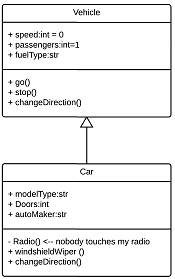
\includegraphics[scale=.7]{Bilder/Klassendiagramm/InteraktionVererbung.png}
%\end{minipage}

\subsubsection{Use-Case-Diagramm (Anwendungsfalldiagramm)}
\label{sec:UseCaseDiagramm}

Quelle: Ionos \cite{IonosUseCase}

\begin{center}
	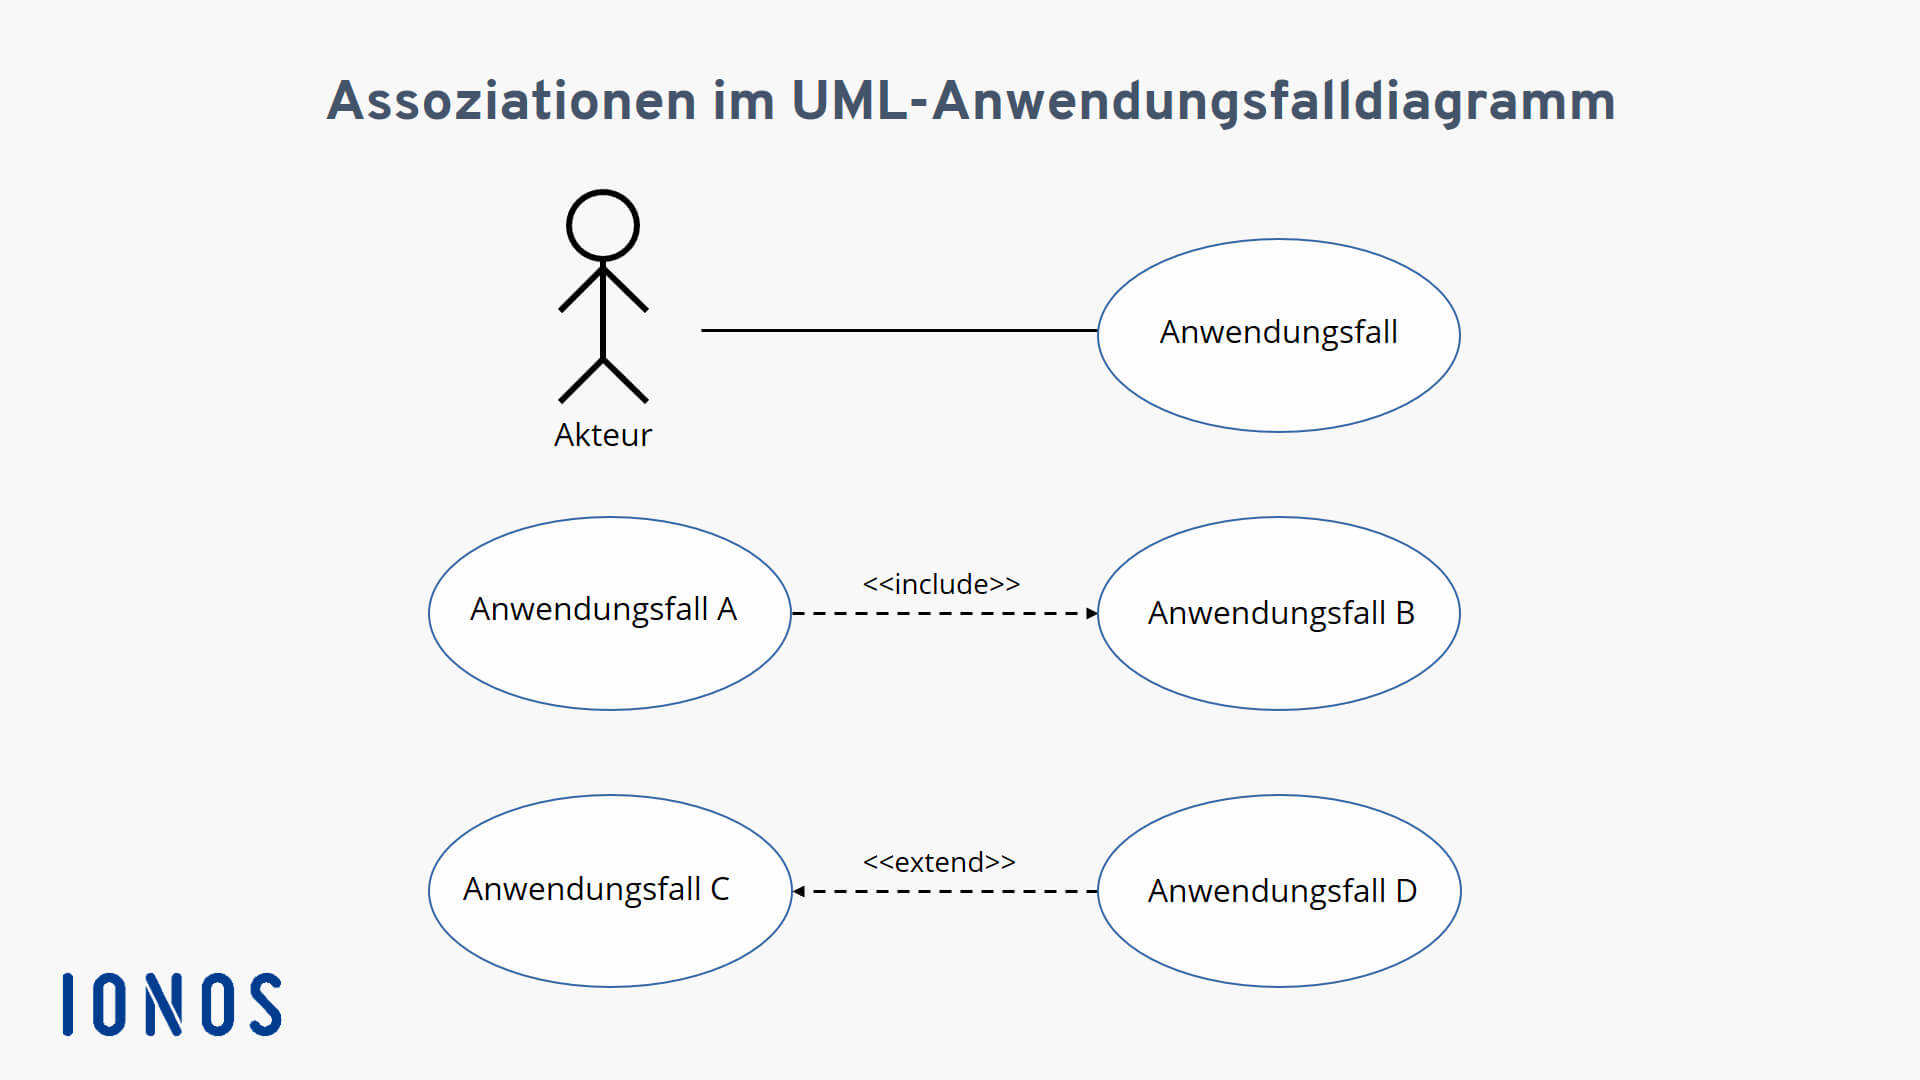
\includegraphics[scale=.25]{Bilder/UseCaseDiagram.png}
	
	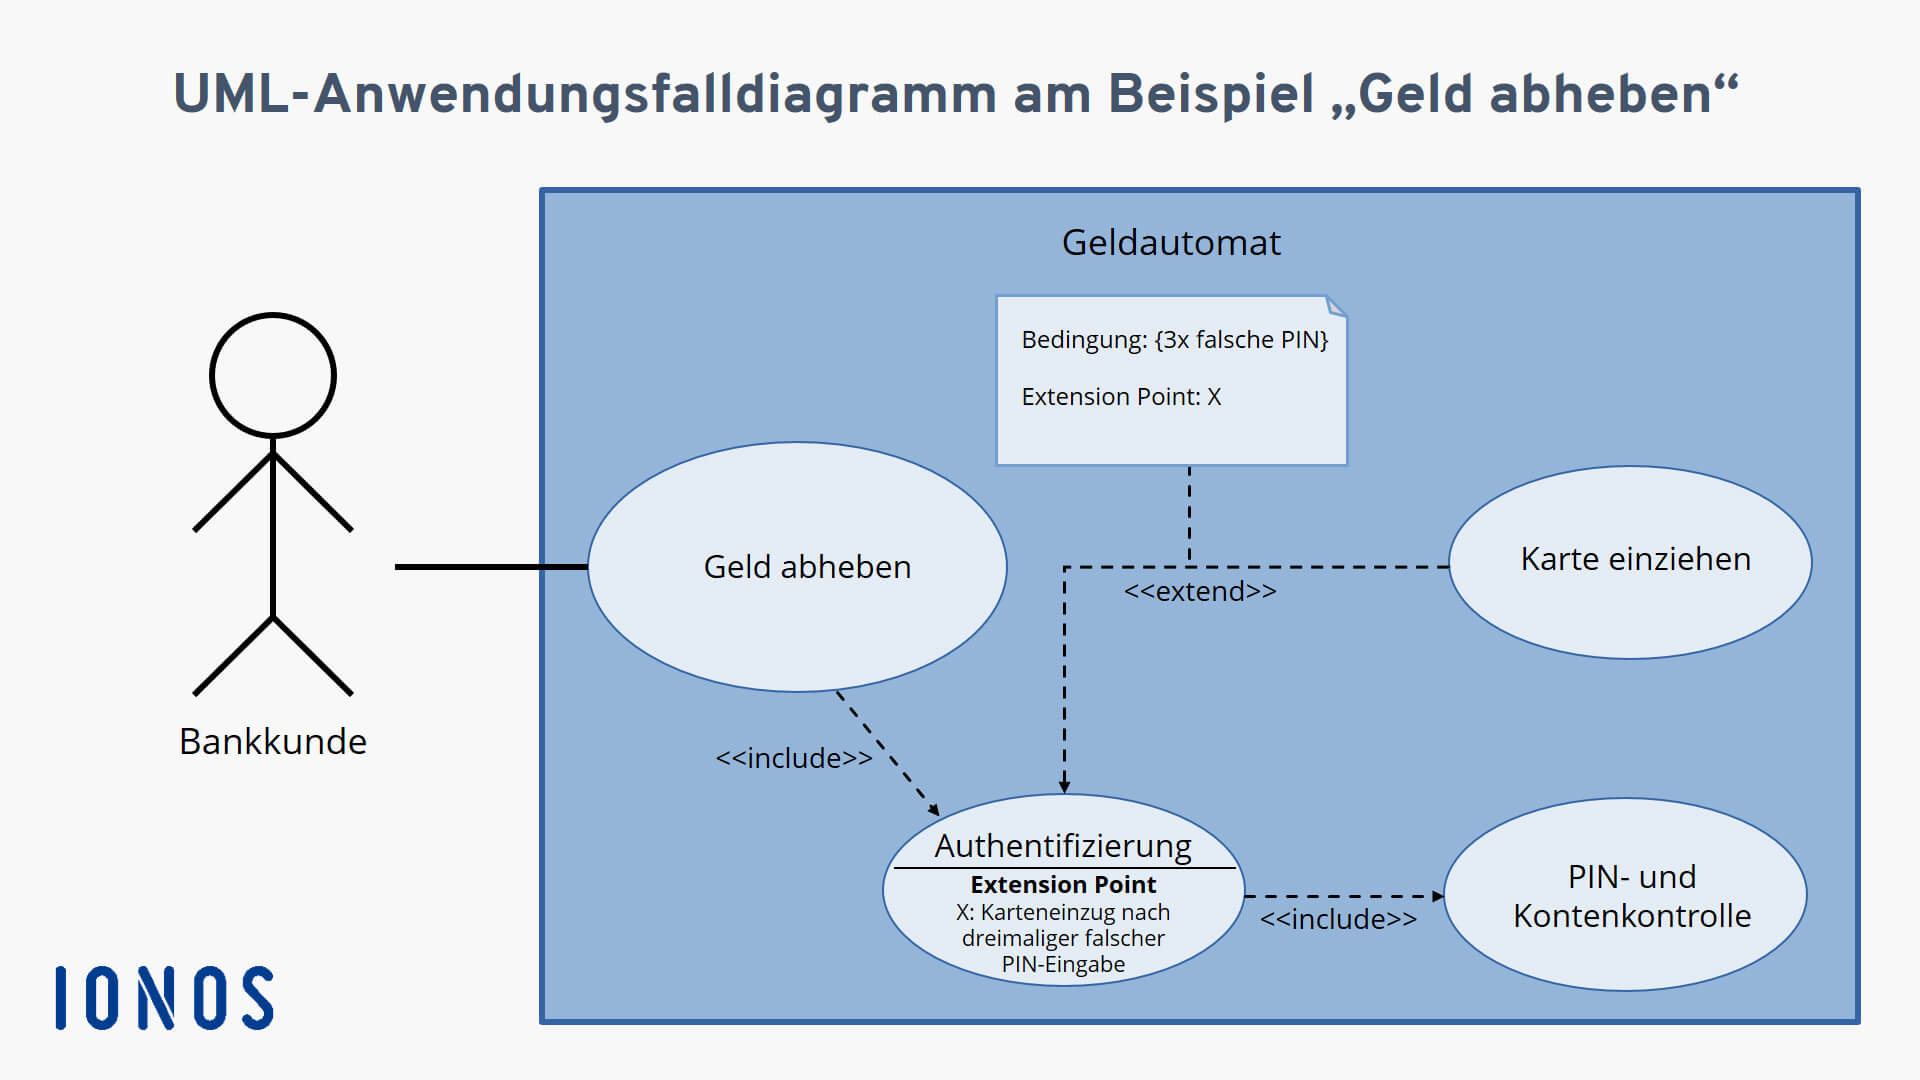
\includegraphics[scale=.25]{Bilder/UseCaseDiagramBeispiel.png}
\end{center}

\subsubsection{Zustandsdiagramm}
\label{sec:Zustandsdiagramm}

\begin{center}
	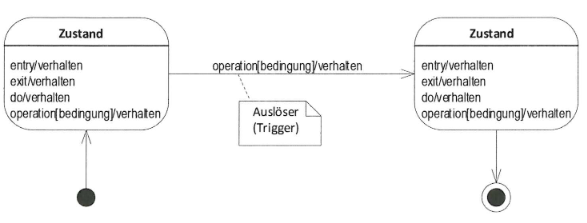
\includegraphics[scale=.9]{Bilder/Zustandsdiagramm.png}
\end{center}

\subsubsection{Aktivitätsdiagramm}
\label{sec:Aktivitaetsdiagramm}

\begin{center}
	\includegraphics[scale=.7]{Bilder/Aktivitätsdiagramm.png}
\end{center}

\subsubsection{Flussdiagramm}
\label{sec:Flussdiagramm}

\begin{multicols}{2}
	\begin{center}
		\begin{tikzpicture}[node distance=1cm]
			\node (start) [startstop] {Start/Ende};
			\node (process) [process, below=of start] {Prozess-/Tätigkeitssymbol};
		\end{tikzpicture}
	\end{center}
	
	\begin{center}
		\begin{tikzpicture}[node distance=1cm]
			\node (io) [io] {Eingabe/Ausgabe};
			\node (decision) [decision, below=0.3cm of process, shape aspect=2] {Entscheidungssymbol};
			\draw [arrow] (io) -- node[anchor=east] {Verbindungspfeil} (decision);
		\end{tikzpicture}
	\end{center}
\end{multicols}

\newpage

\subsubsection{Struktogramm (Nassi-Shneiderman-Diagramm)}
\label{sec:Struktogramm}

Quelle: Lehrerfortbildung-bw.de \cite{Struktogramm}

\begin{minipage}[c]{0.25\textwidth}
Anweisung
\end{minipage}
\begin{minipage}[c]{0.65\textwidth}
	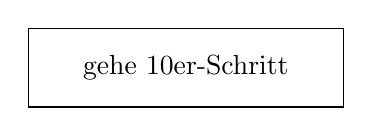
\begin{tikzpicture}[node distance=0cm]
		\node[minimum height=1cm, minimum width=4cm, draw]{gehe 10er-Schritt};
	\end{tikzpicture}
\end{minipage}

\hfill

\begin{minipage}[c]{0.25\textwidth}
	Sequenz
\end{minipage}
\begin{minipage}[c]{0.65\textwidth}
	\begin{tikzpicture}[node distance=0cm]
		\node[minimum height=1cm, minimum width=4cm, draw](10erSchritt){gehe 10er-Schritt};
		\node[minimum height=1cm, minimum width=4cm, draw, below=of 10erSchritt](stift){schalte Stift ein};
		\node[minimum height=1cm, minimum width=4cm, draw, below=of stift](sageHi){sage 'Hallo!'};
	\end{tikzpicture}
\end{minipage}

\hfill

\begin{minipage}[c]{0.25\textwidth}
	Schleife mit Bedingung
\end{minipage}
\begin{minipage}[c]{0.65\textwidth}
	\begin{tikzpicture}[node distance=0cm]
		\node[minimum height=2cm, minimum width=5cm, draw](wiederhole){};
		\node[minimum height=2cm, minimum width=5cm, above=-1.5cm of wiederhole](wiederholeText){wiederhole bis Rand berührt};
		\node[minimum height=1cm, minimum width=4cm, draw, below right=-1cm and -4cm of wiederhole](aendere){ändere x um 10};
	\end{tikzpicture}
\end{minipage}

\hfill

\begin{minipage}[c]{0.25\textwidth}
	Schleife mit Zähler
\end{minipage}
\begin{minipage}[c]{0.65\textwidth}
	\begin{tikzpicture}[node distance=0cm, align=center]
		\node[minimum height=3cm, minimum width=5cm, draw](wiederhole){};
		\node[minimum height=2cm, minimum width=5cm, above=-1.5cm of wiederhole](wiederholeText){wiederhole 10 mal};
		\node[minimum height=1cm, minimum width=4cm, draw, below right=-2.1cm and -4cm of wiederhole](gehe){gehe 4er-Schritt};
		\node[minimum height=1cm, minimum width=4cm, draw, below right=-1.1cm and -4cm of wiederhole](drehe){drehe dich nach rechts\\um 5 Grad};
	\end{tikzpicture}
\end{minipage}

\hfill

\begin{minipage}[c]{0.25\textwidth}
	Endlosschleife
\end{minipage}
\begin{minipage}[c]{0.65\textwidth}
	\begin{tikzpicture}[node distance=0cm, align=center]
		\node[minimum height=3cm, minimum width=5cm, draw](wiederhole){};
		\node[minimum height=2cm, minimum width=5cm, above=-1.5cm of wiederhole](wiederholeText){wiederhole fortlaufend};
		\node[minimum height=1cm, minimum width=4cm, draw, below right=-2cm and -4cm of wiederhole](gehe){gehe 8er-Schritt};
		\node[minimum height=1cm, minimum width=4cm, draw, below right=-1cm and -4cm of wiederhole](drehe){pralle vom Rand ab};
	\end{tikzpicture}
\end{minipage}

\hfill

\begin{minipage}[c]{0.25\textwidth}
	Verzweigung mit \\Alternative
\end{minipage}
\begin{minipage}[c]{0.65\textwidth}
	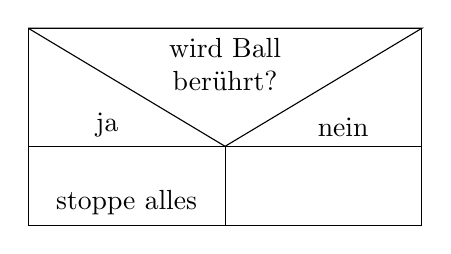
\begin{tikzpicture}[node distance=0cm, align=center]
		\draw (0,0) -- (5,0) node[below,pos=0.5]{wird Ball\\berührt?} -- (2.5,-1.5) -- (0,0);
		\draw (0,0) -- (0,-1.5) -- (2.5,-1.5)node[above,pos=0.4]{ja};
		\draw (0,-1.5) -- (0,-2.5) -- (2.5,-2.5) node[above, pos=0.5]{stoppe alles} -- (2.5,-1.5);
		\draw (5,0) -- (5,-1.5) -- (2.5,-1.5)node[above,pos=0.4]{nein};
		\draw (5,-1.5) -- (5,-2.5) -- (2.5,-2.5) -- (2.5,-1.5);
		
	\end{tikzpicture}
\end{minipage}

\hfill
\newpage

\subsection{Softwarearchitektur}
\label{sec:Softwarearchitektur}

\begin{itemize}
	\item Bottom-Up- und Top-Down-Verfahren bei der Modellierung erläutern
	\item Funktion/Vorteile der Modularisierung von Programmen
	\item Softwarearchitektur
	\begin{itemize}
		\item 3-Schichten-Modell
		\item Model View Controller (MVC)
		\item Model View Presenter (MVP)
		\item Model-View-ViewModel (MVVM)
		\item REST
	\end{itemize}
\end{itemize}

\paragraph{Bottom-Up}

\paragraph{3-Schichten-Modell}

Das 3-Schichten-Modell ist ein Architekturmuster zur Strukturierung von Anwendungen, bei dem die Anwendung in drei Schichten unterteilt wird: die Präsentationsschicht (Presentation Layer), die Logikschicht (Business Logic Layer) und die Datenschicht (Data Layer). Jede Schicht hat eine klar definierte Verantwortung und Aufgabe: Die Präsentationsschicht ist für die Darstellung der Benutzeroberfläche und die Interaktion mit dem Benutzer zuständig, die Logikschicht enthält die Geschäftslogik und die Anwendungslogik und die Datenschicht kümmert sich um den Zugriff auf die Datenbank oder andere externe Datenquellen.

\paragraph{Model View Controller (MVC)}

MVC ist ein Entwurfsmuster zur Strukturierung von Benutzeroberflächen in Softwareanwendungen. Es teilt die Anwendung in drei Hauptkomponenten auf: das Modell (Model), die Ansicht (View) und den Controller. Das Modell repräsentiert die Daten und die Geschäftslogik der Anwendung, die Ansicht ist für die Darstellung der Benutzeroberfläche zuständig, und der Controller nimmt Benutzereingaben entgegen, verarbeitet sie und aktualisiert das Modell und die Ansicht entsprechend.

\paragraph{Model View Presenter (MVP)}

MVP ist ein Variante des MVC-Musters, bei dem der Presenter als Vermittler zwischen dem Modell und der Ansicht fungiert. Der Presenter übernimmt die Aufgabe der Steuerung der Benutzerinteraktionen und der Aktualisierung des Modells und der Ansicht. Im Gegensatz zum MVC-Muster ist die Ansicht im MVP-Muster passiv und enthält keine Logik, was zu einer besseren Trennung von Präsentation und Geschäftslogik führt.

\paragraph{Model View ViewModel (MVVM)}

MVVM ist ein weiteres Entwurfsmuster zur Strukturierung von Benutzeroberflächen, das häufig in der Entwicklung von Desktop- und Webanwendungen verwendet wird. Es ähnelt dem MVP-Muster, aber anstelle eines Presenters wird ein ViewModel verwendet, um die Präsentation der Daten zu steuern. Das ViewModel stellt eine abstrakte Repräsentation der Ansicht dar und erleichtert die Bindung von Daten zwischen dem Modell und der Ansicht.

\paragraph{REST}

REST (Representational State Transfer) ist ein Architekturstil für die Entwicklung von verteilten Systemen, insbesondere Webanwendungen. Es basiert auf dem Prinzip, dass Ressourcen über einheitliche Schnittstellen (URLs) angesprochen und durch die standardisierten HTTP-Methoden (GET, POST, PUT, DELETE) manipuliert werden können. RESTful-Services verwenden keine speziellen Protokolle oder Technologien, sondern nutzen die vorhandenen HTTP-Standards für die Kommunikation zwischen Client und Server.
\subsection{Softwareergonomie}
\label{sec:Softwareergonomie}

\begin{itemize}
	\item Mock-up
	\item Usability vs. User-Experience
	\item Entwurf der Bildschirmausgabemasken (Softwareergonomie, Barrierefreiheit)
	\item Barrierefreiheit bzw. Inklusives Design
\end{itemize}
\subsection{Software Engineering}
\label{sec:SoftwareEngineering}


\subsection{Design Patterns}
\label{sec:DesignPatterns}

\begin{itemize}
	\item Design Patterns kennen/erklären/implementieren
	\begin{itemize}
		\item Singleton
		\item Observer
		\item Factory
		\item Strategy
		\item Decorator
		\item MVC
	\end{itemize}
\end{itemize}
\subsection{Softwarequalität}
\label{sec:Softwarequalitaet}

\begin{itemize}
	\item Software-Qualitätsmerkmale nach ISO 9126 nennen und erläutern
	\begin{itemize}
		\item Funktionalität: Angemessenheit, Interoperabilität, Ordnungsmäßigkeit, Richtigkeit, Sicherheit
		\item Änderbarkeit: Analysierbarkeit, Modifizierbarkeit, Testbarkeit, Stabilität
		\item Übertragbarkeit: Anpassbarkeit, Austauschbarkeit, Installierbarkeit, Koexistenz
		\item Effizienz: Verbrauchsverhalten, Zeitverhalten
		\item Zuverlässigkeit: Fehlertoleranz, Reife, Wiederherstellbarkeit
		\item Benutzbarkeit: Attraktivität, Bedienbarkeit, Erlernbarkeit, Verständlichkeit
	\end{itemize}
	\item Software-Qualitätsmerkmale nach ISO 25010 nennen und erläutern
	\begin{itemize}
		\item Functional Suitability: Functional Completeness, Functional Correctness, Functional Appropriateness
		\item Performance Efficiency: Time Behaviour, Resource Utilization, Capacity
		\item Compatibility: Co-existence, Interoperability
		\item Usability: Appropriateness Recognizability, Learability, Operability, User Error Protection, User Interface Aesthetics, Accessibility
		\item Reliability: Maturity, Availability, Fault Tolerance, Recoverability
		\item Security: Confidentiality, Integrity, Non-repudiation, Authenticity, Accountability
		\item Maintainability: Modularity, Reusability, Analysability, Modifiability, Testability
		\item Portability: Adaptability, Installability, Replaceability
	\end{itemize}
	\item Maßnahmen zur Qualitätssicherung
	\begin{itemize}
		\item Continuous Integration/Delivery/Deployment
	\end{itemize}
\end{itemize}
\subsection{Webentwicklung}
\label{sec:Webentwicklung}

\begin{itemize}
	\item Web 2.0
	\begin{itemize}
		\item Social Networks, Wikis, Blogs, Twitter, Forum, Podcast
	\end{itemize}
	\item Web 3.0
	\item Angriffsmöglichkeiten gegen Anwendungen abgrenzen
	\begin{itemize}
		\item SQL-Injection, Session Hijacking, DoS, DDoS
	\end{itemize}
\end{itemize}